\let\negmedspace\undefined
\let\negthickspace\undefined
\documentclass[journal]{IEEEtran}
\usepackage[a5paper, margin=10mm, onecolumn]{geometry}
\usepackage{lmodern} % Ensure lmodern is loaded for pdflatex
\usepackage{tfrupee} % Include tfrupee package

\setlength{\headheight}{1cm} % Set the height of the header box
\setlength{\headsep}{0mm}     % Set the distance between the header box and the top of the text

\usepackage{gvv-book}
\usepackage{gvv}
\usepackage{cite}
\usepackage{amsmath,amssymb,amsfonts,amsthm}
\usepackage{algorithmic}
\usepackage{graphicx}
\graphicspath{{./figs/}}
\usepackage{textcomp}
\usepackage{xcolor}
\usepackage{txfonts}
\usepackage{listings}
\usepackage{enumitem}
\usepackage{mathtools}
\usepackage{gensymb}
\usepackage{comment}
\usepackage[breaklinks=true]{hyperref}
\usepackage{tkz-euclide} 
\usepackage{listings}
\usepackage{gvv}                                        
\def\inputGnumericTable{}                                 
\usepackage[latin1]{inputenc}                                
\usepackage{color}                                            
\usepackage{array}                                            
\usepackage{longtable}                                       
\usepackage{calc}                                             
\usepackage{multirow}                                         
\usepackage{hhline}                                           
\usepackage{ifthen}                                           
\usepackage{lscape}
\usepackage{circuitikz}
\tikzstyle{block} = [rectangle, draw, fill=blue!20, 
text width=4em, text centered, rounded corners, minimum height=3em]
\tikzstyle{sum} = [draw, fill=blue!10, circle, minimum size=1cm, node distance=1.5cm]
\tikzstyle{input} = [coordinate]
\tikzstyle{output} = [coordinate]
\begin{document}
\bibliographystyle{IEEEtran}
\vspace{3cm}
\title{1.10.7}
\author{EE25BTECH11048-Revanth Siva Kumar.D}
	\maketitle
	% \newpage
	% \bigskip
	{\let\newpage\relax\maketitle}
	
	\renewcommand{\thefigure}{\theenumi}
	\renewcommand{\thetable}{\theenumi}
	\setlength{\intextsep}{12pt} % Space between text and floats
	
	\numberwithin{equation}{enumi}
	\numberwithin{figure}{enumi}
	\renewcommand{\thetable}{\theenumi}
	
	\textbf{Question}:\\
    
         Find a unit vector in the direction of the vector PQ, where P and Q have co-ordinates (5,0,8) and (3,3,2),respectively.
         
         \solution \\
         Given,\\
         The points: 
         \begin{align}
             \vec{P}=\myvec{5\\0\\8} \vec{Q}=\myvec{3\\3\\2}
         \end{align}
         Let the required unit vector be $\vec{x}$, then\\ 
         The formula for unit vector along a line joining two points
         \begin{align}
             \vec{{x}}=\frac{\vec{X}}{\norm{\vec{X}}} \label{unit}
         \end{align}
         The vector along $\vec{P}$ and $\vec{Q}$ is\\
         \begin{align}
             \vec{X}=\vec{Q}-\vec{P} \label{vector}
         \end{align}
         By \eqref{vector}
         \begin{align}
             \vec{X}=\myvec{5\\0\\8}-\myvec{3\\3\\2}
         \end{align}
         \begin{align}
             \vec{X}=\myvec{5-3\\0-3\\8-2}
         \end{align}
         \begin{align}
             \vec{X}=\myvec{2\\-3\\6}
         \end{align}
         Magnitude of the vector $\vec{X}$ is\\
         \begin{align}
             \norm{\vec{X}}=\sqrt{X^T X}
         \end{align}
         \begin{align}
             \norm{\vec{X}}=\sqrt{\myvec{2,-3,6}\myvec{2\\-3\\6}}
         \end{align}
         \begin{align}
             \norm{\vec{X}}=\sqrt{\brak{2}^2+\brak{-3}^2+\brak{6}^2}
         \end{align}
         \begin{align}
             \norm{\vec{X}}=\sqrt{49}
         \end{align}
         \begin{align}
             \norm{\vec{X}}=7
         \end{align}
         Then the unit vector by \eqref{unit},\\
         \begin{align}
             \vec{x}=\frac{1}{7}\vec{X}=\vec{x}=\frac{1}{7}\myvec{2\\-3\\6}
         \end{align}
         \begin{align}
             \vec{x}=\frac{1}{7}\myvec{2\\-3\\6}
         \end{align}
         \begin{align}
             \vec{x}=\myvec{\frac{2}{7},\frac{-3}{7},\frac{6}{7}}
         \end{align}
         Therefore, the required unit vector is\\
         \begin{align}
             \vec{x}=\myvec{\frac{2}{7},\frac{-3}{7},\frac{6}{7}}
         \end{align}
         \begin{figure}
             \centering
             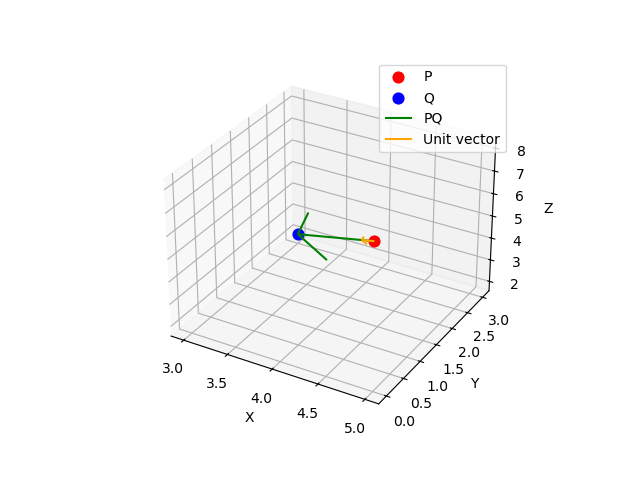
\includegraphics[width=1\columnwidth]{figs/Figure1.png}
             \caption{Plot for the unit vector along PQ using shared output }
             \label{fig:fig21}
         \end{figure}
         \begin{figure}
             \centering
             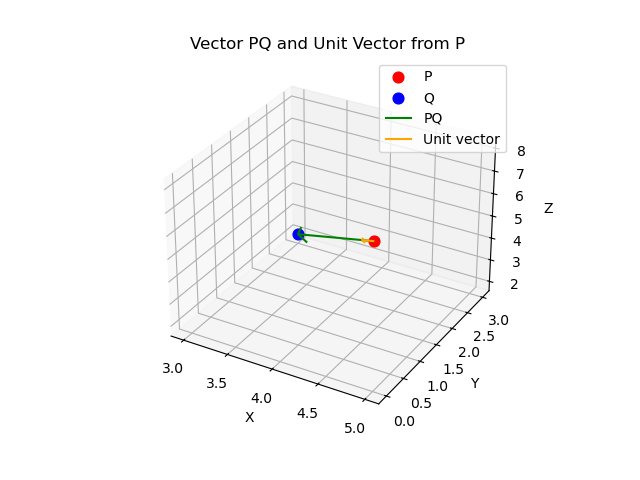
\includegraphics[width=1\columnwidth]{figs/Figure2.png}
             \caption{Plot for the unit vector along PQ using direct python code }
             \label{fig:fig21}
         \end{figure}
         
\end{document}
